\section{2つの円柱のアセンブリ}
このケースでは、2つの円柱からなる単純なアセンブリを解析します。その寸法は:
\begin{itemize}
\item 1本目の円柱の直径:80mm
\item 1本目の円柱の長さ:100mm
\item 2本目の円柱の直径:50mm
\item 2本目の円柱の長さ:120mm
\end{itemize}
円柱は、CADソフトウェアで個別のパーツとしてモデル化され、そのアセンブリをステップ形式でインポートする必要があります。
\begin{enumerate}
\item
  {[}mm, ton, s, °C{]}単位の新規ファイルを作成し、ステップ形式のジオメトリをPrePoMaxにインポートします。
  次に、両方のパーツをメッシュ分割します。
  ここでは、最大要素サイズとして5mmを選択し、その他の設定は変更しませんでした(図\ref{fig:05-01})。
	\begin{figure}[H]
	\centering
	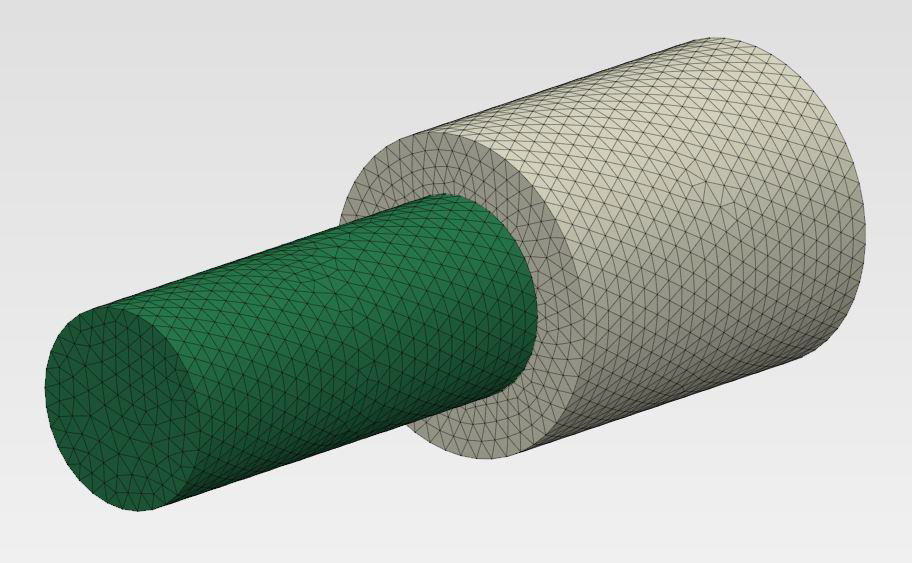
\includegraphics[width=120mm]{fig/05-01.png}
	\caption{2つの円柱 - メッシュ}
	\label{fig:05-01}
	\end{figure}
\vspace{-\baselineskip}
\item
  新しい材料を定義し、弾性挙動を加え、ヤング率を180000MPa、ポアソン比を0.25と指定します。
  先に作成した材料を参照して新しいソリッドセクションを作成し、そのセクションがこのパーツに割り当てられるように円柱を選択します。
\item
  幅の広い円柱を非表示にし、幅の狭い円柱の背面にTie1という名前のサーフェスを作成します。
  パーツの可視性を反転させ(View → Invert Visible Parts)、幅の広い円柱の前面にTie2という名前のサーフェスを作成します。
  再び両方のパーツを表示します。
  タイ拘束を定義し、以前に作成したサーフェスをマスターとスレーブ領域として使用します。
\item
  デフォルトの設定で静的ステップを作成します。
  幅の広い円柱の背面に固定境界条件を適用し、幅の狭い円柱の前面に圧力荷重(大きさ30MPa)を適用します(図\ref{fig:05-02})。
	\begin{figure}[H]
	\centering
	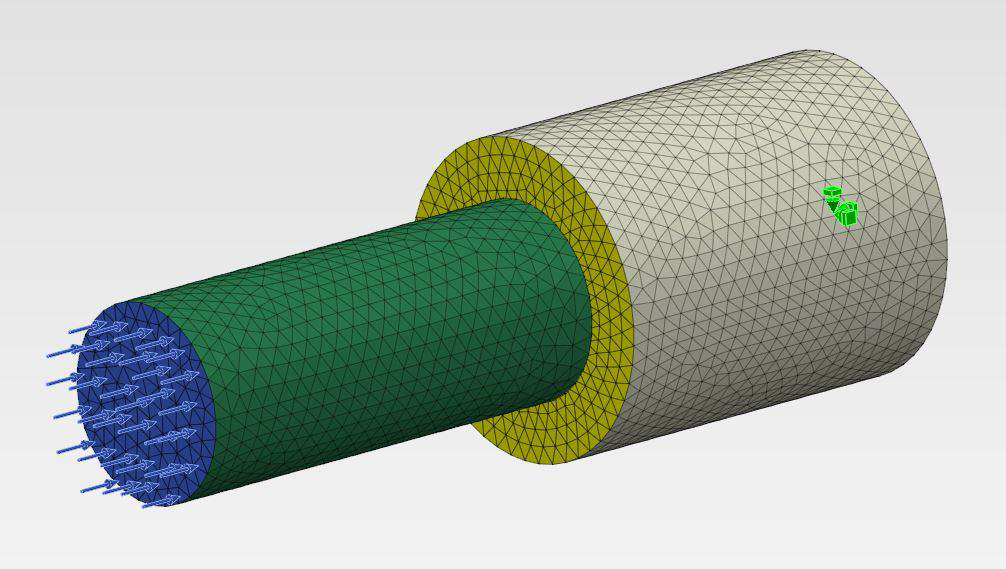
\includegraphics[width=135mm]{fig/05-02.png}
	\caption{2つの円柱 - 境界条件と荷重}
	\label{fig:05-02}
	\end{figure}
\vspace{-\baselineskip}
\item
  解析を実行し、結果を表示します。変形のスケール係数を100として、応力と変位を調べます(図\ref{fig:05-03})。
	\begin{figure}[H]
	\centering
	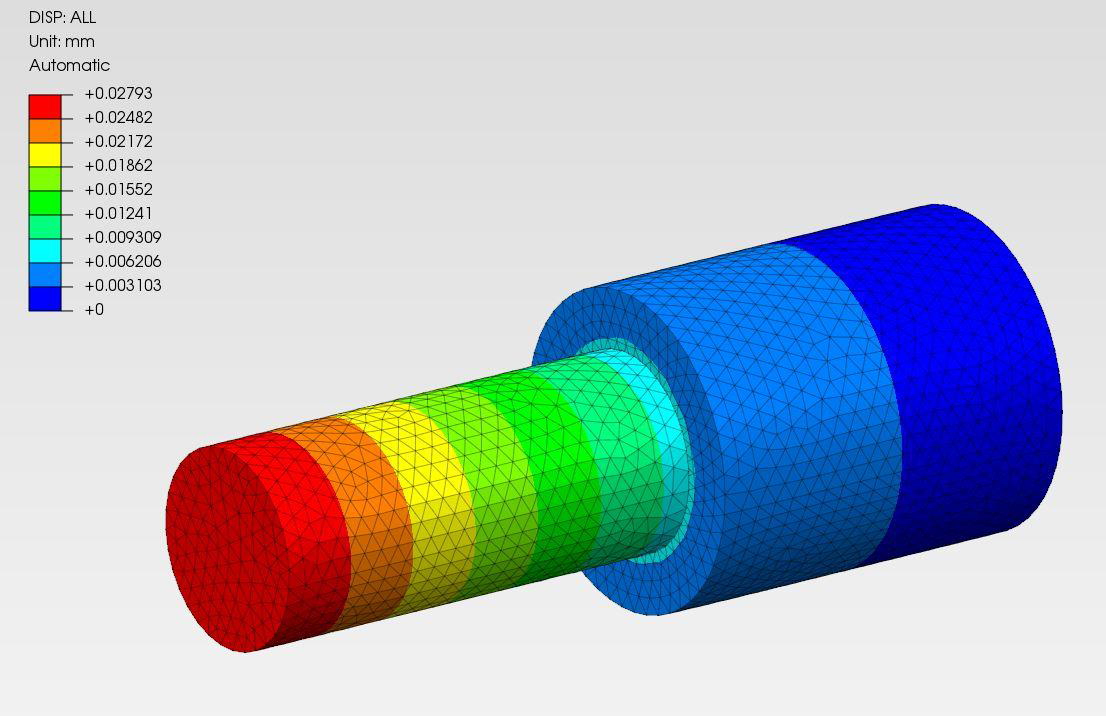
\includegraphics[width=135mm]{fig/05-03.png}
	\caption{2つの円柱 - 変位}
	\label{fig:05-03}
	\end{figure}
\vspace{-\baselineskip}
\end{enumerate}